\title{Registers}
\begin{document}
\section{Registers}

\begin{frame}{Registers}
  \begin{definition}
    A \alert{register} is a collection of two or more D flip-flops that use a common clock signal.
  \end{definition}
  Registers can be used for a number of purposes, including:
  \begin{itemize}
    \item Storage of common data in a CPU, like an address
    \item Control but settings
  \end{itemize}
\end{frame}

\begin{frame}{The 74x175 4-bit register}
  \begin{columns}
    \begin{column}{6cm}
      \begin{center}
        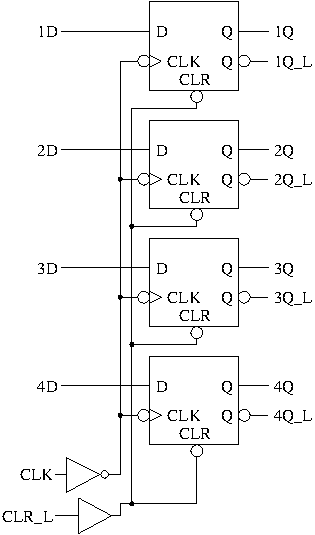
\includegraphics[scale=0.7]{74x175Logic}
      \end{center}
    \end{column}
    \begin{column}{6cm}
      \begin{center}
        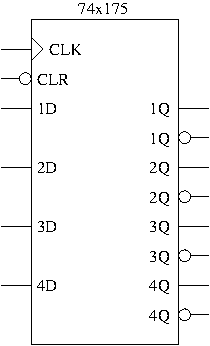
\includegraphics[scale=0.7]{74x175Schematic}
      \end{center}
    \end{column}
  \end{columns}
\end{frame}

\section{Latches}

\begin{frame}{The other kind of latch}
  An MDI \alert{latch} is similar to a register, except that it uses D latches instead of flip-flops.
  \begin{itemize}
    \item The clock input is replaced by an enable input.
    \item When the enable is asserted, the outputs are constantly changing to match the inputs.
    \item When the eneable is not asserted, the last inputs are ''latched`` to the outputs and held until the enable is asserted.
  \end{itemize}
\end{frame}

\begin{frame}{The 74x373 latch}
  \begin{center}
    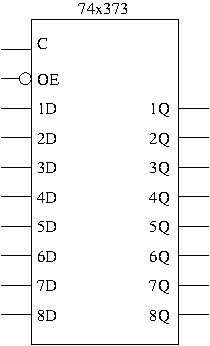
\includegraphics{74x373Schematic}
  \end{center}
\end{frame}

\end{document}
